\documentclass[10pt,xcolor={dvipsnames}]{beamer}
\usepackage{polyglossia}
\usepackage{mathtools, amsthm, amssymb, amsfonts}
\usepackage{graphicx}
\setdefaultlanguage{french}
\usepackage{listings}
\usepackage{lstautogobble}

\usefonttheme{professionalfonts}
\usepackage{unicode-math}

\setmathfont{Latin Modern Math}
%\setmathfont[range={it}]{Latin Modern Sans 10 Oblique}
\setmathfont[range=up]{Latin Modern Sans}
\setmathfont[range={\mathbb}]{xits-math.otf}
%\setmathfont{xits-math.otf}
\setmonofont[Mapping=tex-text,Scale=0.9]{Consolas}

\lstset{language=Python,
	escapechar=\%,
	basicstyle=\ttfamily,
	keywordstyle=\color{OliveGreen}\ttfamily,
	stringstyle=\color{red}\ttfamily,
	commentstyle=\color{brown}\ttfamily,
	morecomment=[l][\color{blue}]{\#},
	columns=fixed,
	tabsize=4,
	autogobble=true
	keepspaces=false
}

%\usetheme{Frankfurt}
\usetheme{Hannover}
\usecolortheme{dolphin}

\newcommand{\N}{\mathbb N}
\newcommand{\Z}{\mathbb Z}
\newcommand{\R}{\mathbb R}
\newcommand{\Q}{\mathbb Q}
\newcommand{\CC}{\mathbb C}
\newcommand{\K}{\mathbb K}
\DeclarePairedDelimiter{\intcc}{[\![}{]\!]}

\newcounter{Exercice}
\resetcounteronoverlays{Exercice}
\makeatletter
\newenvironment{exo}[1][\@nil]{
	\def\tmp{#1}
	\refstepcounter{Exercice}
	\begin{block}{\textbf{Exercice \theExercice}
			\ifx\tmp\@nnil
			%
			\else
			(#1)
			\fi
		}
	}{\end{block}}
\makeatother

\newcounter{Exemple}
\resetcounteronoverlays{Exemple}
\makeatletter
\newenvironment{exem}[1][\@nil]{
	\def\tmp{#1}
	\refstepcounter{Exemple}
	\begin{block}{\textbf{Exemple \theExemple}
			\ifx\tmp\@nnil
			%
			\else
			(#1)
			\fi
		}
	}{\end{block}}
\makeatother

\title{Atelier d'informatique}
\subtitle{\textbf{Épisode V:} Tracés avec \lstinline|matplotlib|}

\begin{document}

\begin{frame}
	\titlepage
\end{frame}

\frame{\tableofcontents}

\setlength\parskip{0.8em}
\section{Introduction}

\begin{frame}[fragile]{Introduction}
	La librairie \lstinline|matplotlib| permet de créer des graphes scientifiques en Python, tels que des courbes représentatives de fonctions, des histogrammes, des diagrammes en boîte, ou encore des nuages de points.\pause
	
	On ne s'intéressera ici qu'au tracé de courbes représentatives de fonctions.\pause
	
	Pour toute la suite du cours, veillez à ce que votre script contienne les lignes suivantes\pause
	\begin{lstlisting}
		import matplotlib.pyplot as plt
		import numpy as np
	\end{lstlisting} et qu'il ait été exécuté au moins une fois.
\end{frame}

\subsection{Principe}

\begin{frame}[fragile]{Introduction}{Principe}
	La librairie \lstinline|matplotlib| crée des objets qui permettent de manipuler des figures, de type \lstinline|Figure|, qui contiennent des zones de tracé, de type \lstinline|Axes|, dans lesquels se situent des tracés, de type \lstinline|Line2D| le plus souvent.\pause
	
	Utiliser \lstinline|matplotlib| pour effectuer un tracé revient à définir une figure, une zone de tracé, puis à faire le tracé dans la zone.
\end{frame}

\begin{frame}[fragile]	
	On peut le faire de manière interactive, en tapant des instructions directement dans la console, sans stocker chaque objet dans une variable: \lstinline|matplotlib| comprend automatiquement qu'il doit se référer au dernier objet créé, dans la dernière figure créée.\pause
	
	Quand on utilise un script, il est conseillé de manipuler directement les objets et utiliser les méthodes qui sont définies dessus. Par souci de simplicité, on fera sans.
\end{frame}

\section{Utilisation}

\subsection{Définir une figure}

\begin{frame}[fragile]{Utilisation}{Définir une figure}
	Pour définir un objet \lstinline|figure|, on utilise le constructeur associé, \lstinline|plt.figure|. Il fonctionne comme une fonction, donc il faut mettre des parenthèses:\pause
	\begin{lstlisting}
		plt.figure()
	\end{lstlisting}
	\pause
	et on peut éventuellement préciser le numéro de la figure à créer en mettant un nombre entier entre les parenthèses.
	\pause
	En mode interactif, la zone de tracé est définie \textbf{automatiquement} lorsque l'on effectue un tracé. \lstinline|matplotlib| le définit alors dans la figure la plus récente.
\end{frame}

\subsection{Effectuer un tracé}

\begin{frame}[fragile]{Utilisation}{Effectuer un tracé}
	Étant donné une liste \lstinline|X| des \textit{abscisses} et une liste \lstinline|Y| des \textit{ordonnées} correspondante l'on veut tracer, il suffit d'utiliser l'instruction
	\begin{lstlisting}
		plt.plot(X,Y)
	\end{lstlisting} 
	pour effectuer le tracé.
	
	Pour afficher, on utilise l'instruction \lstinline|plt.show()|.
\end{frame}

\begin{frame}[fragile]
	\begin{exem}
	Le code
		\begin{lstlisting}
			X = [0,1,2]
			Y = [6,10,3]
			plt.figure()
			plt.plot(X,Y)
		\end{lstlisting}
	produit la figure suivante (en affichant avec \lstinline|plt.show()|):
	\begin{figure}
		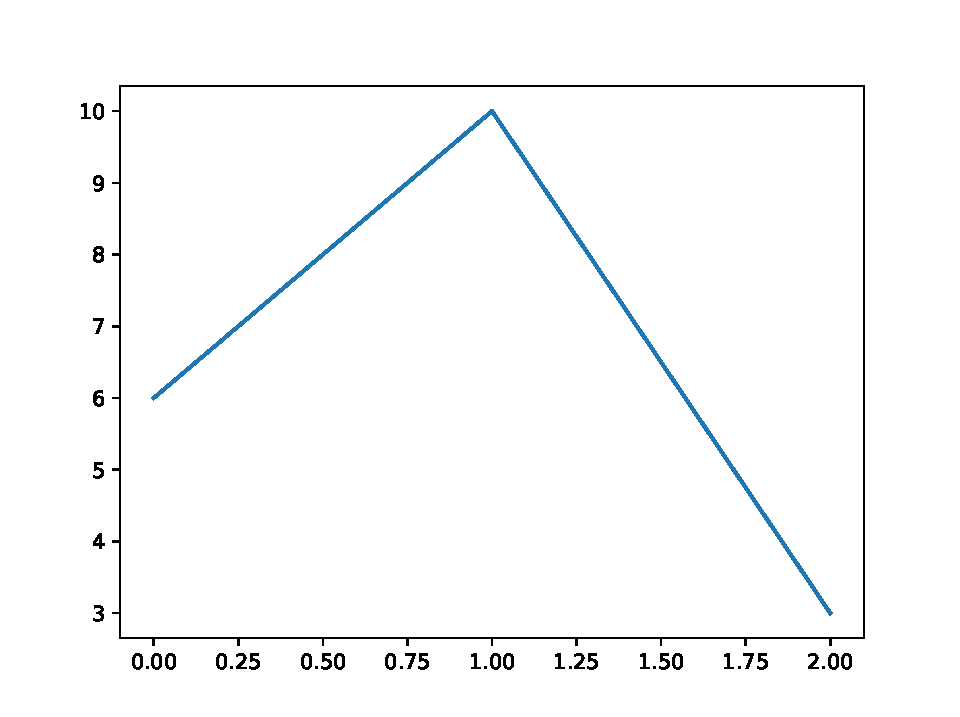
\includegraphics[height=0.5\textheight]{exemple_matplotlib_1.pdf}
	\end{figure}
	\end{exem}
\end{frame}

\section{Tracer le graphe d'une fonction compliquée}

\begin{frame}[fragile]{Tracer le graphe d'une fonction compliquée}
	Étant donnée une fonction numérique (qui renvoie des valeurs) \lstinline|f| et un intervalle $I$ sur lequel on veut tracer son graphe, il nous faut d'abord représenter par une liste de points l'intervalle.\pause
	
	Pour cela, la librairie \lstinline|numpy| nous fournit une fonction nommée \lstinline|linspace|. On l'utilise de la façon suivante:
	\begin{lstlisting}
		X = np.linspace(a, b, N)
	\end{lstlisting}
	où \lstinline|a| et \lstinline|b| sont les extrémités de l'intervalle $I$ (par exemple $-3$ et $2$ si $I=[-3,2]$), et \lstinline|N| le nombre de points avec lequel on veut représenter $I$. Le plus il y en a, le plus fidèle sera la courbe tracée.\pause
	
	Enfin, on effectue l'instruction \lstinline|Y = f(X)| pour calculer les ordonnées, et on fait comme décrit avant.
\end{frame}

\begin{frame}[fragile]
	\begin{exem}[$x\mapsto\frac{1}{x^2}$]
		\begin{lstlisting}
			def f(x):
				return 1/(1+x**2)
			X = np.linspace(-2,2,200)
			Y = f(X)
			plt.figure()
			plt.plot(X,Y)
			plt.grid()
		\end{lstlisting}
	\begin{figure}
		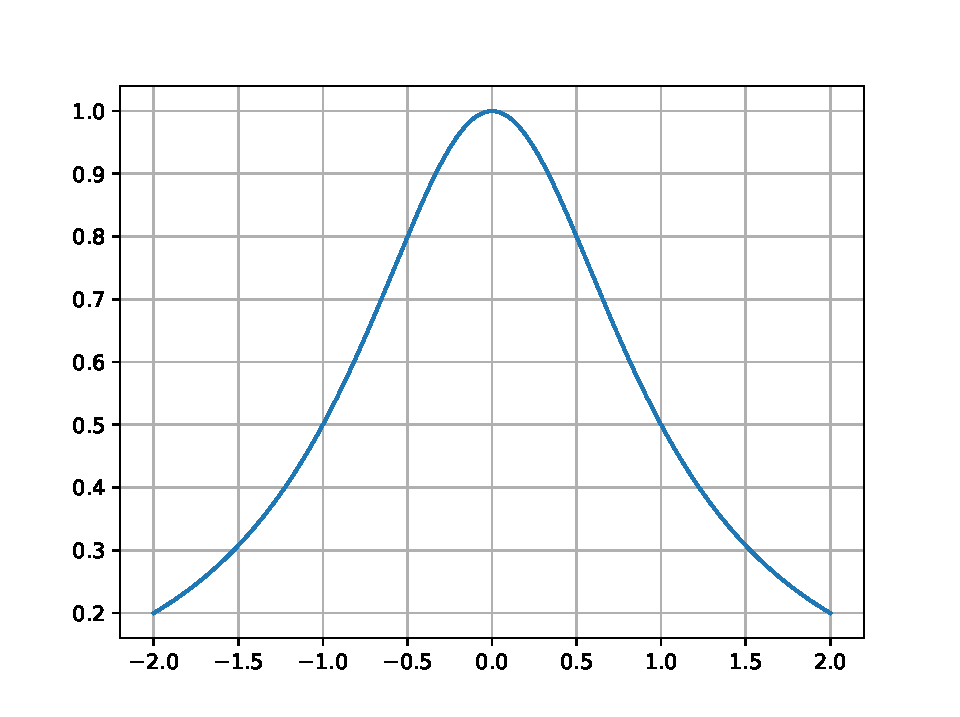
\includegraphics[height=0.5\textheight]{exemple_matplotlib_2.pdf}
	\end{figure}
	\end{exem}
\end{frame}

\section{Des options multiples}

\begin{frame}[fragile]{Des options multiples}
	Pour ajouter un quadrillage au repère, on peut utiliser \lstinline|plt.grid|. C'est une méthode relative à dernière zone de tracé en mémoire, donc on lui fait appel via \lstinline|plt.grid()|. Elle fonctionne comme un interrupteur, ajoute un quadrillage s'il n'y en a pas, l'enlève s'il y en a déjà un. On peut forcer l'ajout en précisant \lstinline|plt.grid(True)|.\pause
	
	On peut donner un titre au graphe via \lstinline|plt.title|, qui est aussi une méthode, à laquelle on fait appel en passant pour argument la chaîne de caractère que l'on veut utiliser comme titre:
	\begin{lstlisting}
		plt.title("La meilleure courbe du monde. Vraiment.")
	\end{lstlisting}\pause
\end{frame}

\begin{frame}[fragile]{Des options multiples}
	On peut également forcer à occuper le plus d'espace possible en utilisant la méthode \lstinline|tight_layout|: \lstinline|plt.tight_layout()| essaie de minimiser les espaces vides sur la figure.\pause
	
	Il existe encore plein d'options, que l'on peut trouver dans la documentation de \lstinline|matplotlib| (attention, c'est en anglais...).
\end{frame}
\end{document}